\documentclass[tikz,border=10pt]{standalone}
\usetikzlibrary{calc}
\begin{document}
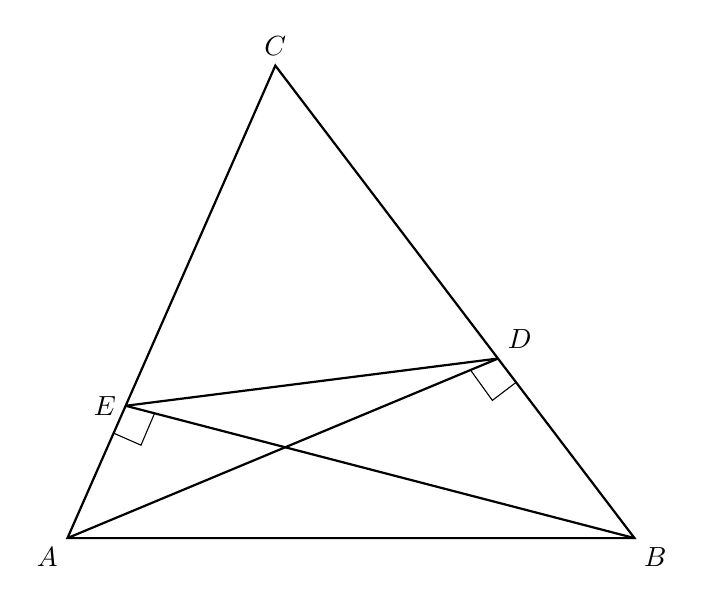
\begin{tikzpicture}[scale=1.2]
  \coordinate (A) at (0,0);
  \coordinate (B) at (6,0);
  \coordinate (C) at (2.2,5);
  % D on CB such that AD is perpendicular to CB
  \coordinate (D) at ($(C)!0.62!(B)$);
  % E on AC such that BE is perpendicular to AC
  \coordinate (E) at ($(C)!0.72!(A)$);
  \draw[thick] (A) -- (B) -- (C) -- cycle;
  \draw[thick] (A) -- (D);
  \draw[thick] (B) -- (E);
  \draw[thick] (D) -- (E);
  % right angle mark at D (between DB and DA)
  \draw ($(D)!9pt!(B)$) -- ($($(D)!9pt!(B)$)!9pt!90:(D)$) -- ($(D)!9pt!(A)$);
  % right angle mark at E (between EA and EB)
  \draw ($(E)!9pt!(A)$) -- ($($(E)!9pt!(A)$)!9pt!-90:(E)$) -- ($(E)!9pt!(B)$);
  \node[below left] at (A) {$A$};
  \node[below right] at (B) {$B$};
  \node[above] at (C) {$C$};
  \node[above right] at (D) {$D$};
  \node[left] at (E) {$E$};
\end{tikzpicture}
\end{document}
